\section{Descripción general del entorno de pruebas}
Para las pruebas se generaron aleatoriamente 25 puntos de control que fueron distribuidos
geograficamente de forma aleatoria y no uniforme en un área de total de $3,028 km^{2}$. En los 25
puntos de control fueron distribuidos un total de 1.146 individuos en un estado inicial de larvas.

El periodo de simulación utilizado fue igual a 50 días con 10 temperaturas constantes :
15\textcelsius , 18\textcelsius , 20\textcelsius , 22\textcelsius , 24\textcelsius , 25\textcelsius
, 26\textcelsius , 27\textcelsius , 30\textcelsius , 34\textcelsius. La dirección al igual que la
temperatura fue establecida como una constante para las pruebas, cuyo valor fue la dirección
suroeste, que genera un ángulo que varía entre $202,5^{\circ}$ a $247,5^{\circ}$.

Los parámetros del simulador del proceso evolutivo, en su mayoría son calculados con datos
biológicos correspondientes al área de estudio. Obtener dichos datos requieren minuciosos estudios
de campo que escapan del alcance de este trabajo.

En cuanto a los sitios de reproducción, los parámetros $bs_{min}$ y $bs_{max}$ fueron
configurados según lo observado en \cite{otero2006stochastic, otero2008stochastic}, siendo $15$ y
$50$ los valores adoptados respectivamente.  El valor de $bs_{med}$ fue establecido, en $32,5$,
realizando un promedio entre $bs_{min}$ y $bs_{max}$.

Los coeficientes para el modelo simplificado de Sharpe y DeMichele, con inhibición de altas
temperaturas de Schoolfield, para el calculo de las tasas de desarrollo media en $dias^{-1}$,
fueron tomados de :  \cite{rueda1990temperature} para el desarrollo larvario y el desarrollo
pupal, y de  \cite{otero2006stochastic} para la eclosión de huevos, ciclo gonotrófico para hembras
nulíperas y paridas.

\section{Resultados y discusión}

En general, para todos los casos, la población inicial sufre un decrecimiento causada por la
mortalidad diaria de los individuos a temperaturas entre 15 y 34 \textcelsius, y por la emergencia
de adultos a temperaturas entre 18 y 34 \textcelsius. La aparición de adultos implica que la
población de individuos en etapas inmaduras (huevos, larvas y pupas), llegaron a completar su
ciclo de desarrollo para dar lugar a mosquitos adultos, por lo tanto la población de individuos en
etapas inmaduras tiende a disminuir y mientras que la población de mosquitos adultos tiende a
aumentar. El crecimiento de la población se debe a que las hembras adultas pertenecientes a la
población de mosquitos, culminaron su ciclo gonotrófico y dieron lugar la ovipostura.


\begin{figure}[!t]
    \centering
    \begin{subfigure}[b]{0.45\textwidth}
        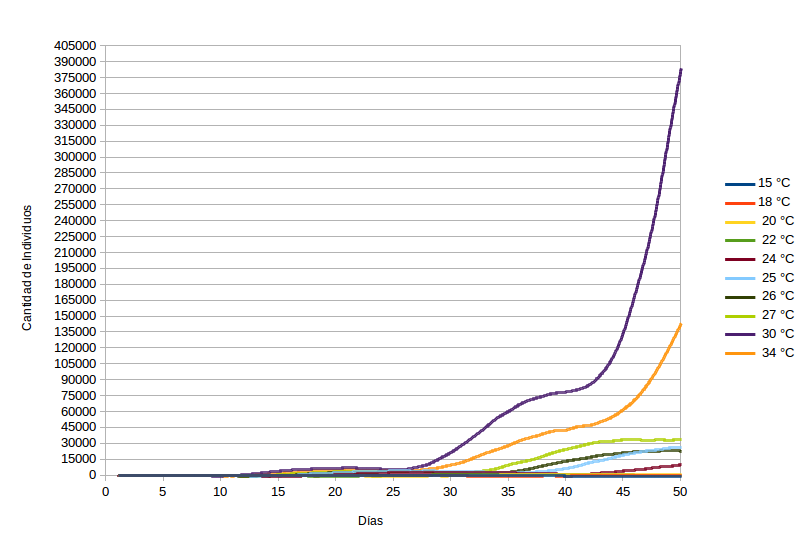
\includegraphics[width=\textwidth]{./graphics/evolucion-poblacion-all.png}
        \caption{ Población de mosquitos en etapas inmaduras.}
    \end{subfigure}
    ~~~~
    \begin{subfigure}[b]{0.45\textwidth}
        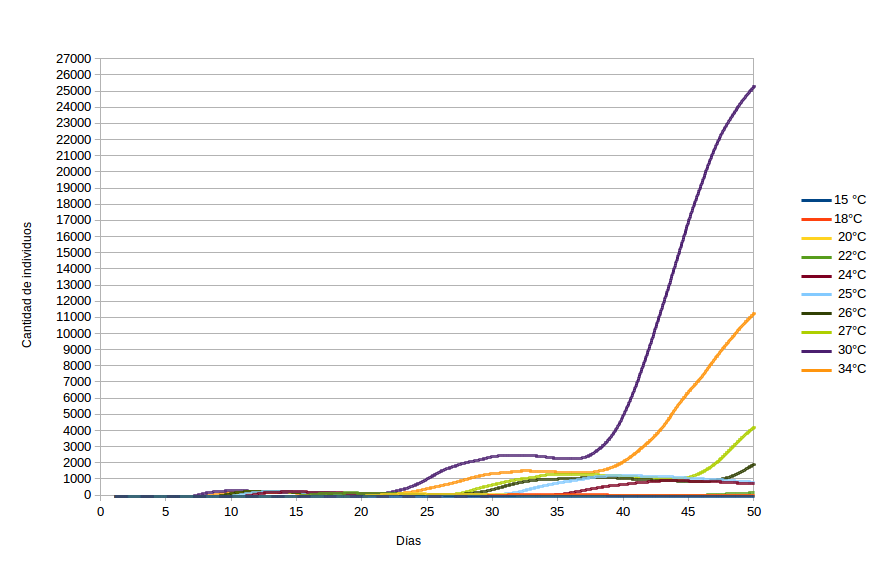
\includegraphics[width=\textwidth]{./graphics/evolucion-poblacion-adultos.png}
        \caption{ Población mosquitos adultos.}
    \end{subfigure}

\caption{\label{fig:poblacion-all}Análisis del comportamiento de la población de mosquitos en relación al tiempo a 10 temperaturas constantes (15-34 \textcelsius)}
\end{figure}

En la \figref{fig:poblacion-all} se puede apreciar el crecimiento y decrecimiento de la población
a diferentes temperaturas, en donde se pudo observar que a medida que la temperatura aumenta, las
tasas de desarrollo son menores, motivo por el cual las poblaciones de individuos en etapas
inmaduras, sometidos a temperaturas más elevadas, tienden a disminuir su tamaño rápidamente debido
a que se desarrollan con mayor rapidez, dando lugar a su etapa de adulto. Del mismo modo el ciclo
gonotrófico, para las hembras adultas tienden a disminuir su duración, causando que el intervalo
entre oviposturas disminuya, en consecuencia el tamaño de la población de individuos en etapas
inmaduras aumenta rápidamente.

\begin{figure}[!t]
    \centering
    \begin{subfigure}[b]{0.225\textwidth}
        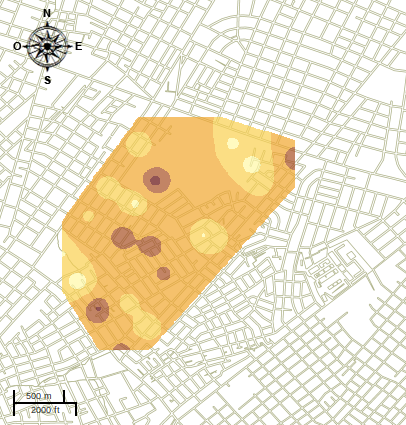
\includegraphics[width=\textwidth]{./graphics/inicial.png}
        \caption{ Población población inicial.}
    \end{subfigure}
    ~~~~
    \begin{subfigure}[b]{0.225\textwidth}
        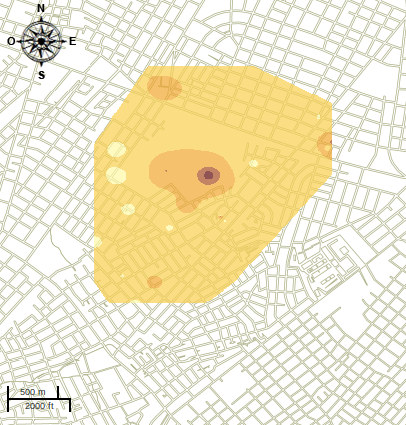
\includegraphics[width=\textwidth]{./graphics/temp-20-final.png}
        \caption{ Población final a 20 \textcelsius.}
    \end{subfigure}

    \begin{subfigure}[b]{0.225\textwidth}
        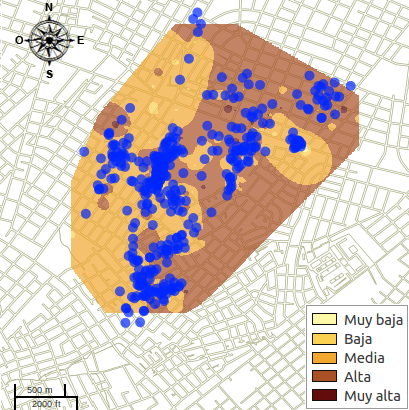
\includegraphics[width=\textwidth]{./graphics/temp-24-final.png}
        \caption{ Población final a 24 \textcelsius.}
    \end{subfigure}
    ~~~~
    \begin{subfigure}[b]{0.225\textwidth}
        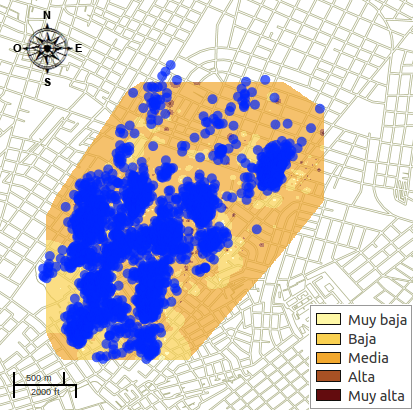
\includegraphics[width=\textwidth]{./graphics/temp-27-final.png}
        \caption{ Población final a 27 \textcelsius.}
    \end{subfigure}

    \begin{subfigure}[b]{0.225\textwidth}
        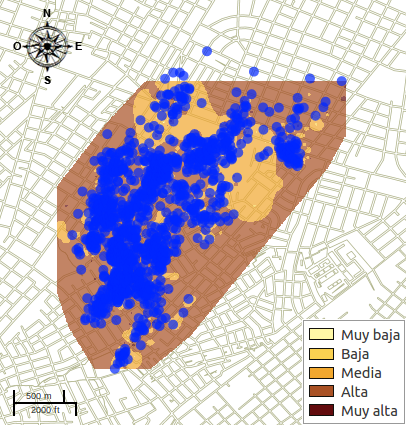
\includegraphics[width=\textwidth]{./graphics/temp-30-final.png}
        \caption{ Población final a 30 \textcelsius.}
    \end{subfigure}
    ~~~~
    \begin{subfigure}[b]{0.225\textwidth}
        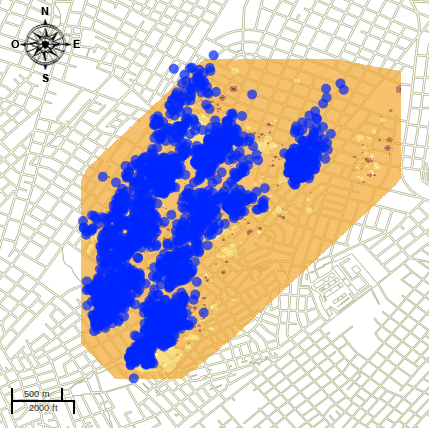
\includegraphics[width=\textwidth]{./graphics/temp-34-final.png}
        \caption{ Población final a 44 \textcelsius.}
    \end{subfigure}
\caption{\label{fig:poblacion-mapas-all} Mapas de interpolación de la población de mosquitos y la distribución de las hembras adultas (puntos en azul).}
\end{figure}

En la \figref{fig:poblacion-mapas-all} se puede apreciar los mapas de interpolación de las
poblaciones en un su estado inicial y final del periodo de simulación. El estado inicial es el
mismo para todas las temperaturas. Comparando el estado inicial y los estados finales se puede
observar que existe una dispersión de los focos en dirección al noreste debido a que la dirección
del viento utilizada era de sureste. Este patrón de dispersión se podrá observar en todas las
poblaciones que fueron sometidas a temperaturas que permitan la generación de hembras adultas. La
dispersión de los focos de infestación es consecuencia de la dispersión y ovipostura de las
hembras adultas emergentes de la población.

